\documentclass[journal=jacsat,manuscript=article]{achemso}
%Image-related packages
\usepackage{graphicx}
\usepackage{subcaption}
\usepackage[export]{adjustbox}
\usepackage{wrapfig}

%%\listfiles

\newcommand*\mycommand[1]{\texttt{\emph{#1}}}

\author{Nayanika Das}
\affiliation[UVicUCC]{Computational Biochemistry and Biophysics Lab, Research Group on Bioinformatics and Bioimaging (BI$^2$), Department of Biosciences, Universitat de Vic - Universitat Central de Catalunya, 08500 Vic, Spain}
\author{Vijay Baladhye}
\affiliation[SPPU]{Savitribai Phule Punr University, Pune, India}
\author{Jordi Villà-Freixa}
\email{jordi.villa@uvic.cat}
\affiliation[UVicUCC]{Computational Biochemistry and Biophysics Lab, Research Group on Bioinformatics and Bioimaging (BI$^2$), Department of Biosciences, Universitat de Vic - Universitat Central de Catalunya, 08500 Vic, Spain}
\alsoaffiliation{IRIS-CC}


\title[Evolutionary trends of GPX6 $\Delta G^{\ddagger}$]
  {Computational Free Energy Directed Evolution In Enzyme Design: Exploring Mutational Pathways With Lower Activation Penalty in Glutathione Peroxidase 6 Homologs}

\abbreviations{IR,NMR,UV}
\keywords{Ancestral enzyme reconstruction, enzyme design, empirical valence bond, free energy calculations}

\usepackage{graphicx} % Required for inserting images
\title{Computational analysis of the evolution of glutathione peroxidase 6 (GPX6) activation free energy}
\begin{document}
\maketitle 

\begin{abstract}
  
\end{abstract}

\section{Introduction}

Selenium (Se), in the form of selenocysteine (Sec, U—the 21st amino acid) occurs in 25 proteins in the human proteome. Insertion of Sec into a protein is much more complicated than the other 20 amino acids because a UGA stop codon must be recoded as a sense codon for Sec \cite{Hondal2011}. The complexity of this process signifies that Sec must fulfill a chemical function that exerts biological pressure on the genome to maintain the Sec-insertion machinery \cite{Hondal2011} \cite{Cardey2007}. The view of Sec as a sophisticated innovation implies that for each occurrence of Sec in an enzyme there is a unique and specific reason for the use of Se to enhance the enzymatic reaction relative to that of S \cite{Hondal2011}. The view of Sec as a sophisticated innovation implies that for each occurrence of Sec in an enzyme there is a unique and specific reason for the use of Se to enhance the enzymatic reaction relative to that of S \cite{Hondal2011}. This view also implies that since Se “speeds reactions” Sec should have widely substituted for Cys in enzymes, which clearly has not occurred. Specific reasons for the usage of Sec might include the enhanced nucleophilic character of Se relative to S, or another might be the much lower pKa of a selenol relative to that of a thiol \cite{Hondal2011}. Although the catalytic triad of glutathione peroxidase (GPX) has been well recognized, there has been little evidence for the relevance of the interactions among the triad amino acid, i.e. selenocysteine (U), glutamine (Q), and tryptophan (W). Hence, the mechanism of has been studied in various aspects. GPXSec activity classically reduces hydroperoxides, particularly hydrogen and lipid peroxides, with glutathione (GSH) as a cofactor \cite{Rees2024}. GPXCys  containing proteins act on alternative substrates for peroxidation and may have additional functions, including signalling and oxidative protein folding. Thus, all GPX proteins may protect cells from oxidative stress \cite{Rees2024}. 

\subsection{Mechanism of GPX}

A catalytic mechanism proposed for GPX3 by Morokuma et al. based on DFT calculations has the resting state of Sec as selenol as shown in the above figure. In the first part of this reaction, hydrogen peroxide coordinates to the active site of the enzyme and the proton transfer is happening to the Gln83 residue \cite{Prabhakar2006} \cite{Prabhakar2005}. Morokuma \cite{Prabhakar2006} did an ONIOM(QM:MM) method to evaluate the quantitative effect of the protein surroundings on the energetics of an enzymatic reaction.  In the first step, the formation of the selenolate anion \({\ Se^-}\) occurs via the proton transfer from the Se through the oxygen (O1) atom of hydrogen peroxide to the neighboring Gln83, leading to the intermediate (III). \cite{Prabhakar2006} The computed barrier for the creation of the selenolate anion is 16.4 kcal/mol. \cite{Prabhakar2006} In the second step of the stepwise mechanism, the O1-O2 bond of $\ce{H_2O_2$ is cleaved. During this process, one hydroxyl fragment (O1H) is transferred to the selenolate anion \({\ Se^-}\) to form selenenic acid (R-SeO1H), while simultaneously the second hydroxyl fragment (O2H) accepts the previously transferred proton from Gln83 to form a water molecule (IV). Overall barrier (from II to IV) for the formation of selenenic acid (E-Se-OH) becomes 18.0 kcal/mol. \cite{Prabhakar2006}

\begin{figure}[h]
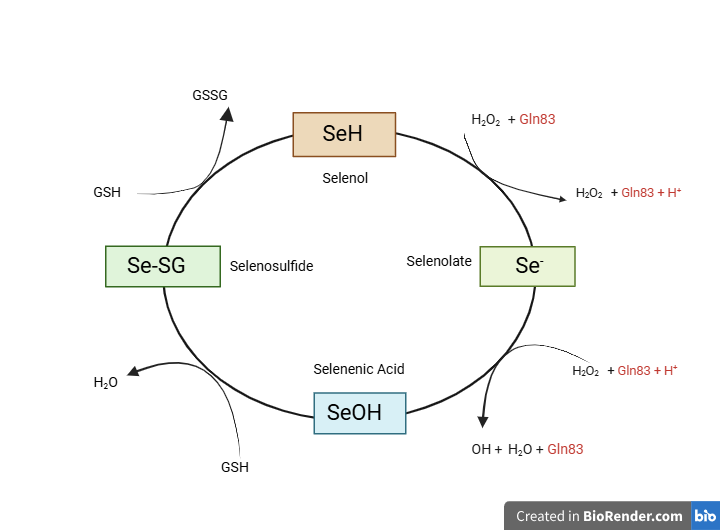
\includegraphics[width=0.7\textwidth, inner]{figures/Catalytic_cycle.png}
\caption{Catalytic Cycle of GPX as given by Morokuma et al. where the resting state of selenium is Selenol}
\label{fig:figure1}
\end{figure}

\begin{wrapfigure}{h}{0.7\textwidth}
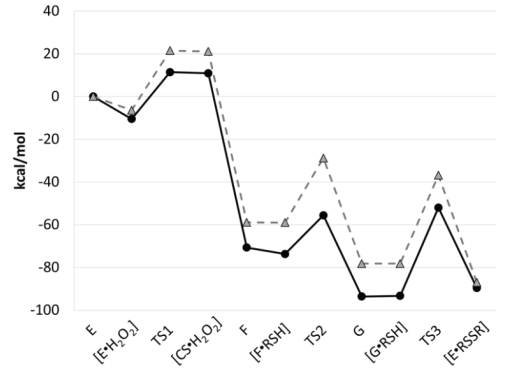
\includegraphics[width=0.7\linewidth]{figures/flohe_energyprofile.png} 
\caption{Energetic profile of the cycle for a SecGPX and the corresponding Cys, as DFT-calculated}
\label{fig:figure2}
\end{wrapfigure}

\begin{figure}[h]
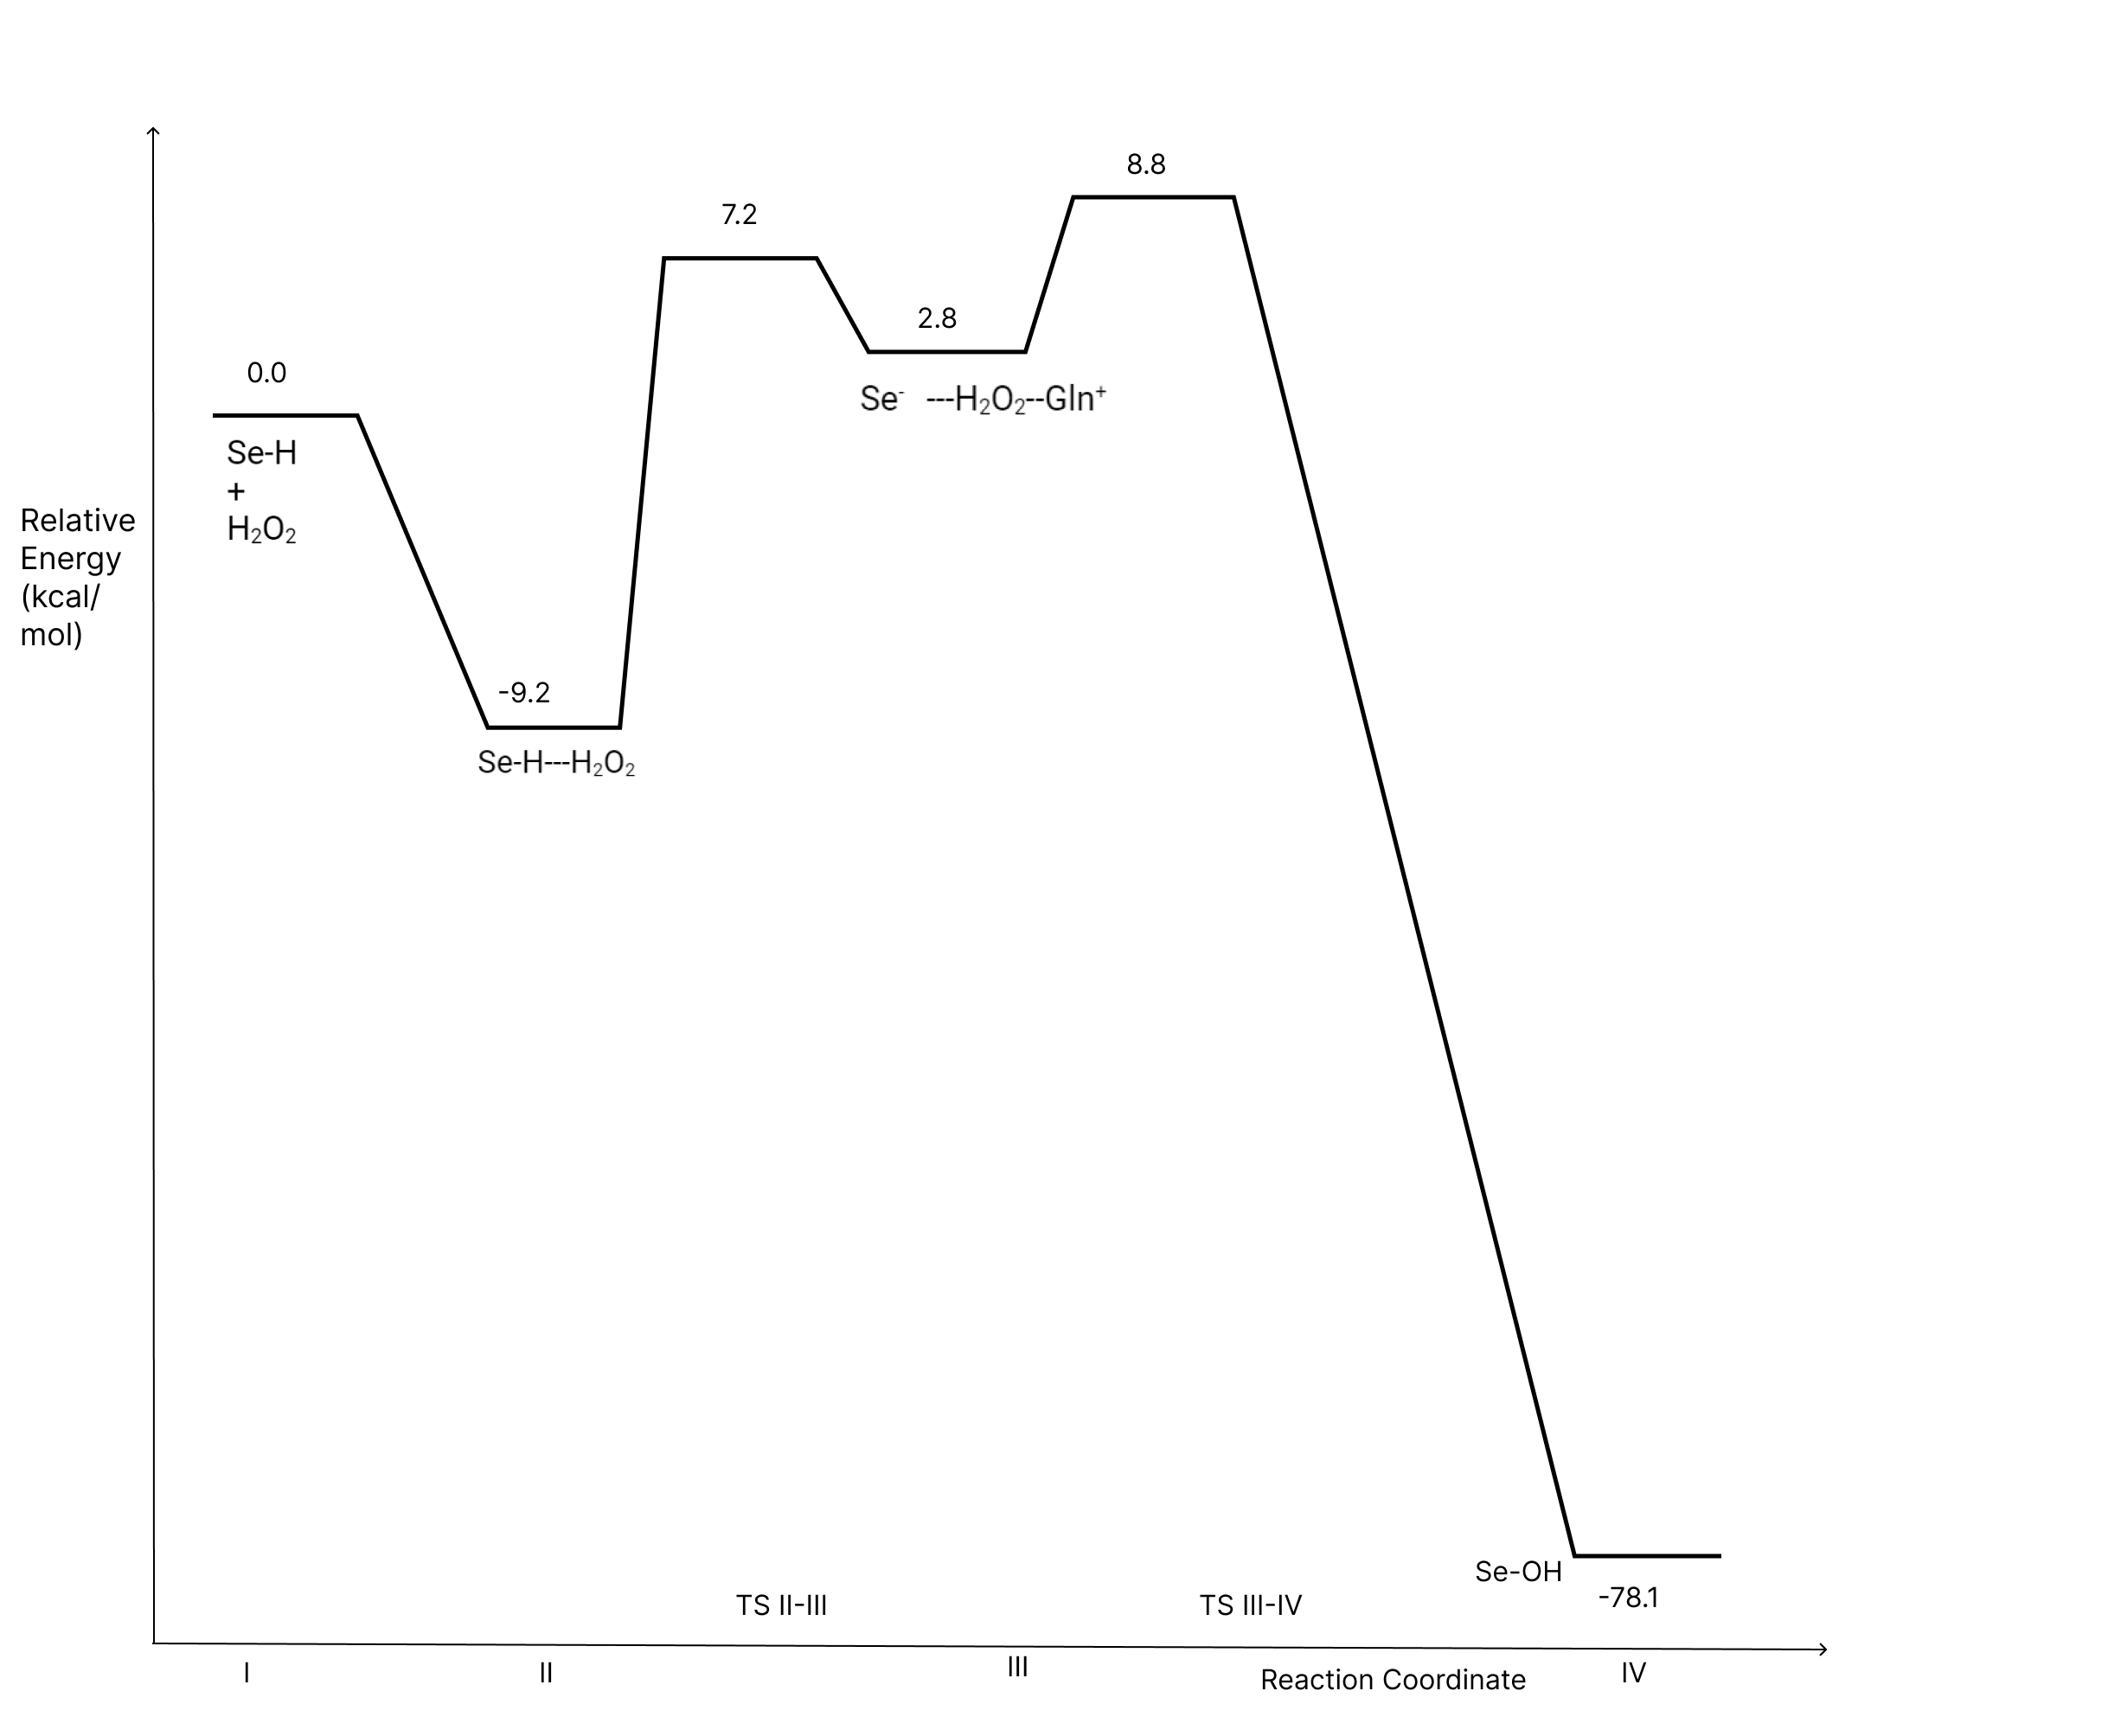
\includegraphics[width=0.7\textwidth, inner]{figures/morokuma_energy_profile.png}
\caption{Potential Energy Diagram for the hydrogen peroxide reduction mechanism by GPX by Morokuma et al.}
\label{fig:figure3}
\end{figure}

Flohe et al \cite{Orian2015} explored the mechanism in a different way wherein the selenocysteine proton moves via water to the indol nitrogen of the Trp residue and then the hydrogen peroxide and with the result of formation of  the products are instantly. They show essentials of the DFT-calculated oxidation of SecGPx by $H_{2} O_{2}$. The calculation was performed with E, as shown in the figure, but with a single water molecule and $H_{2} O_{2}$ bound to the reaction center. \cite{Orian2015} The transition state, leading to the charge-separated form CS, involves three concurrent steps. CS evolves to the selenenic form F and a water molecule. \cite{Orian2015} Formation of the charge separated form does not depend on binding of $H_{2} O_{2}$ but just on the presence of water. Binding of $H_{2} O_{2}$ to CS then generates the identical unstable CS•$H_{2} O_{2}$ complex which decays as described. \cite{Orian2015} In the transition state (TS1), the selenol proton moves via $H_{2} O_{2}$ and water to the Trp nitrogen, thus creating a charge-separated species. The resulting complex [CS•$H_{2} O_{2}$] is so unstable that it decays without any energy barrier. In G the selenocysteine is thiylated by a thiol substrate. \cite{Orian2015}

\subsection{Empirical Valence Bond Model based on the QM/MM calculations}

We come to a hybrid QM/MM method using the empirical valence bond (EVB) which has proven to be very useful for calculating thermodynamic activation parameters for chemical reactions \cite{Oanca2024}. Certainly EVB can capture the changes in the environment around the protein, with the simple force field description and not a large DFT or QM/MM cluster, giving an idea of how the enzyme proceeds to work under certain environmental conditions \cite{Oanca2024}. If the activation free energy is correctly predicted at a given temperature, this just means that the sum of \(\Delta {H^}\) and \(-T\Delta {S^}\) is correctly predicted. A recent change that has been made is for cases where the reference reaction would be rather complex to parameterize the EVB potential energy surface directly on DFT calculations \cite{Oanca2024}. To understand the origin of the thermodynamic activation parameters in the EVB model, it is necessary to understand the basis of EVB. EVB approach is construction of potential energy surfaces. Any number of such states can in principle be used, but often a simple two-state model is considered for an elementary chemical reaction step. The system is then represented by a n × n EVB Hamiltonian \cite{Oanca2024}.

\[ 
  \left[ {\begin{array}{cc}
    H_{11} & H_{12} \\
    H_{21} & H_{22} \\
  \end{array} } \right]
\]
Here, $ H_{11} $ and $ H_{22} $ are the energies of the two valence states which are calculated using classical force fields. The off-diagonal matrix elements represent the coupling between the two states.  The value of the coupling term $ H_{11} $, needs to be calibrated on a reference reaction and there is also a second parameter that must be calibrated and it is phase independent, \cite{Oanca2023} the alpha shift, which corresponds to the constant difference in free energy between the reacting values in the two states. \cite{Oanca2023} These reference values (EVB parameters) are either devised from experimental data, commonly in aqueous solution, or directly by QM/MM calculations on the enzyme. 

\subsection{The Concept of Epistasis and Protein Sequence}

As proteins evolve, they follow trajectories through sequence space, so this topology also determines how mutation, drift, selection, and other forces can drive genetic and functional evolution. Catalytic residues are largely conserved in enzymes as they lower the activation energy of reactions and thereby can increase enzymatic turnover \cite{Rees2024}. Epistasis can cause a mutation that confers or improves a function in one protein to have no effect or even be strongly deleterious in a related protein, attempts to give rise to natural sequence variation.\cite{Starr2016} So, now the question is how prevalent is epistasis within proteins.\cite{Starr2016} One way to gain insights into this in the context of protein evolution is to compare the effects of some mutation when it is introduced into different proteins related by evolutionary homologs.\cite{Starr2016} This is because protein homologs point to both strong and pervasive effects of epistasis that cause the functional effects of mutations to differ between related proteins.\cite{Starr2016} Epistatic interactions between mutant sites can help in explaining why evolution follows certain pathways.\cite{Storz2018} Hence, in this study we focus on selenoprotein Glutathione Peroxidase 6 (GPX6) homologs, essentially mouse and human, exploring the replacement for the rare amino acid Selenocysteine (Sec) to Cysteine (Cys) in Human and Cysteine (Cys) to Selenocysteine (Sec) in Mouse. The goal of this article was to calculate the activation free energy barrier for the Glutathione Peroxidase 6 homologs using Empirical Valence Bond simulation, in order to determine the significant barrier difference with the change in the active site residue from cys/sec. And further more showing analysis on the affect of the catalytic activity of both due to variants imposing environmental changes inside the protein.

\begin{figure}
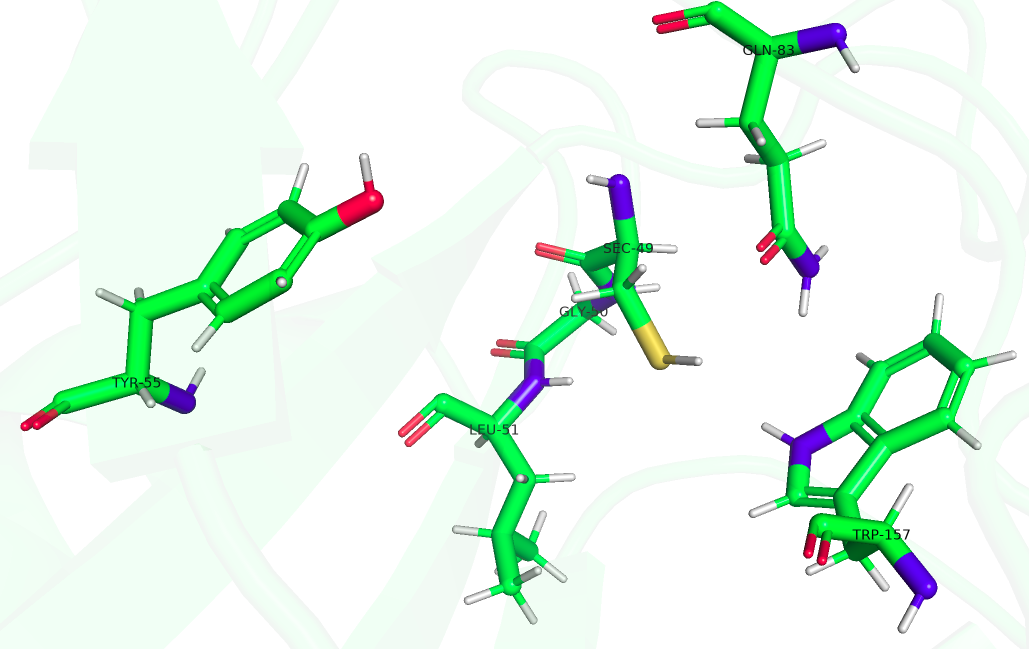
\includegraphics[width=0.7\linewidth]{figures/activesite_humansec.png} 
\caption{Active Site of GPX6 Human}
\label{fig:figure4}
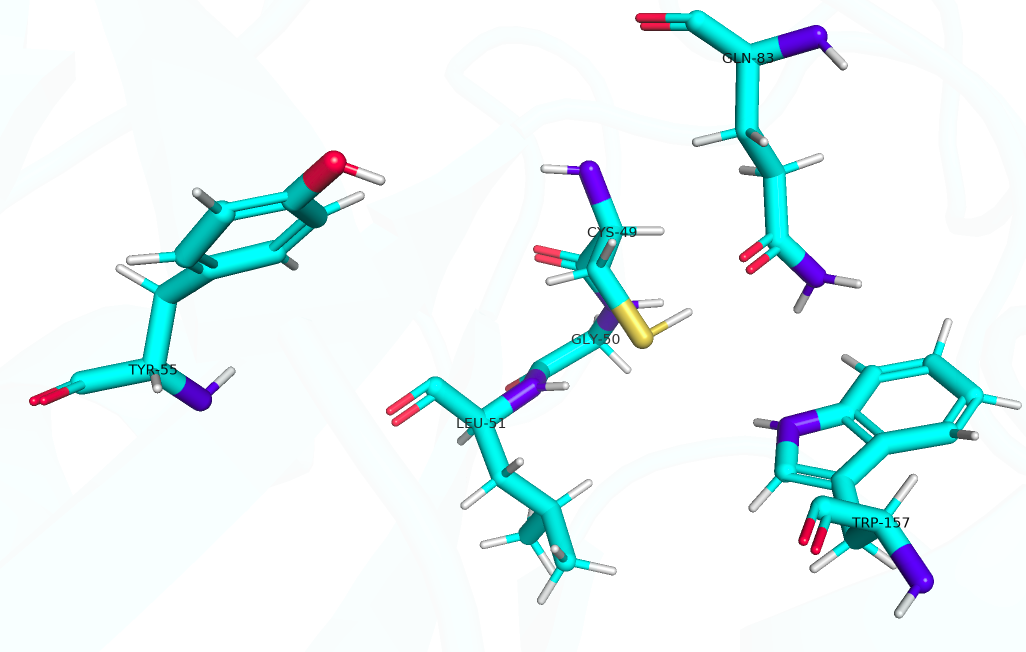
\includegraphics[width=0.7\linewidth]{figures/activesite_mousecys.png} 
\caption{Active Site of GPX6 Mouse}
\label{fig:figure5}
\end{figure}

Active site of GPX contains SEC49 in human GPX6 and CYS49 in mouse GPX6. While they are surrounded by residues GLN83, TRP157, LEU51, TYR55, GLY50. These residues are highly conserved in all GPX isoforms and take an important part in the mechanism. The most feasible mechanism that we followed in this article is the SeH-Gln83 by using the implementation of the DFT calculated reference reaction previously done by Morokuma et al. \cite{Prabhakar2006} to set up our EVB calculations.

\begin{document}

\section{Selection of Variants}

To guide the selection of mutations for directed evolution, a multiple sequence alignment was performed between the human and mouse wild-type protein. This MSA revealed 47 positions that differed between the human and mouse sequences, suggesting potential sites for mutagenesis. In order to prioritize residues for mutagenesis, the distances from the alpha carbon of Cys/Sec49 (active site residue) and rest of the 46 positions were calculated. Residues were then grouped into distance criteria of <10 Å, 10-15 Å, 15-20 Å, 20-25 Å, 25-30 Å, and 30-35 Å. This distance-based approach allowed us to select residues within different proximity ranges to Cys/Sec49. Grouping residues into distance bins provides a systematic and stochastic way to explore the impact of mutations at varying distances from the target residue (Cys/Sec49). We have mutated all these residues one by one slowly changing the human into mouse and the mouse into human structure, in order to understand the changes in the activation barrier in going from proximal to distal mutations in both the structures.

\section{Computational Model Preparation}

The initial structure used to make the EVB model for mouse cysteine wild type was (PDB ID - 7FC2) and for human selenocysteine wild type it was generated with Alphafold. The parametrization includes in preparing a simulation that has missing force field parameters along with standard parameters and library files. In this case, it is Selenium (U). After equilibration, continuing with the FEP simulations which constitute the core part of the EVB methodology. For creating the selenium parameters (selenol, selenolate ion and selenenic acid), FFLD in Maestro was used. We used the charges provided by Maestro; the hydrogen and solvent were added using the Q program \cite{Marelius1999}. The TIP3P water parameters were used in combination with the other protein parameters not present in the standard OPLS library in Q.

\subsection{Free Energy Calculation Using Q}

Free energy perturbation (FEP) calculations with Q involve running a set of consecutive input files which have the mapping parameter $\lambda$ ranging in a way (usually [1, 0] to [0, 1] between two states). Qfep is a program which reads the energy files generated by Qdyn and calculates the total change in free energy for the complete perturbation from state A ($\varepsilon_1$) to state B ($\varepsilon_2$). Zwanzig’s formula as shown below calculates the difference in free energy between the two states:

\begin{equation}
    \Delta G = \sum \Delta g = \sum -R \cdot T \cdot \ln \left\langle e^{-\left(\frac{\Delta V_{\text{eff}}}{R \cdot T}\right)} \right\rangle_{A}
\end{equation}

Here, \(\Delta V_{\text{eff}}\) is defined as the difference in \( V_{\text{eff}} \) between two adjacent perturbation steps. 

Qfep also calculates free energy functions, or potentials of mean force, using the perturbation formula. The reaction coordinate \(X\) is defined as the energy gap between the states \(X = \Delta V = \varepsilon_1 - \varepsilon_2\) and is divided into intervals \(X_m\) (bins). The first term in the equation represents the free energy difference between the initial state \(\varepsilon_1\) and the mapping potential \(V_i\):

\begin{equation}
    \Delta G(X_m) = \Delta G (\lambda_i) - R \cdot T \cdot \ln \left\langle e^{-\left(\frac{E_g(X_m) - V_i(X_m)}{R \cdot T}\right)} \right\rangle_{i}
\end{equation}

The second term represents the free energy difference between the mapping potential \(V_i\) and the ground state potential \(E_g\). The average in this term is taken over those configurations where \(X\) belongs to \(X_m\).

\begin{equation}
    \Delta G(\lambda_i) = - R \cdot T \cdot \ln \left( \sum_{n=0}^{i-1} \left\langle e^{-\left(\frac{V_{n+1} - V_n}{R \cdot T}\right)} \right\rangle_{n} \right)
\end{equation}

\(E_g\) is the solution to the secular determinant. The system is then represented by an \(n \times n\) EVB Hamiltonian.

\[ 
  \left[\begin{array}{cc}
    H_{11} & H_{12} \\
    H_{21} & H_{22} \\
  \end{array}\right]
\]

Here, \(H_{11}\) and \(H_{22}\) are the energies of the two valence states which are calculated using classical force fields. 
For a two-state representation, the solution becomes:

\begin{equation}
    E_g = \frac{1}{2} \cdot \left( \epsilon_1 + \epsilon_2 \right) - \frac{1}{2} \sqrt{ \left( \epsilon_1 - \epsilon_2 \right)^2 + 4 \cdot H_{12}^2 }
\end{equation}

where \(H_{ij}\) or \(H_{12}\) is the off-diagonal matrix element representing the quantum mechanical coupling of the states. \(H_{ij} \neq 0\) results in the mixing of states \(i\) and \(j\). In Qfep, the off-diagonal element \(H_{ij}\) is a function of the form:

\begin{equation}
    H_{ij} = A_{ij} \cdot e^{-(\mu (r_{ij} - r_0) + \eta (r_{ij} - r_0)^2)}
\end{equation}

The EVB method allows calibration of simulated reference reactions to experimental data obtained from gas-phase or solution experiments. The two EVB parameters \(H_{ij}\) (mostly \(A_{ij}\)) and \(\Delta \alpha\) are adjusted in a way until the calculated profile and the experimental data coincide. The \(\Delta \alpha\) parameter determines the \(\Delta G^\circ\) level, and \(H_{ij}\) regulates the degree of mixing of the states at the transition state, i.e., the \(\Delta G^\ddagger\) level.

\subsection{EVB simulations}

Spherical boundary conditions \cite{King1989} were applied to the system using Q program \cite{Marelius1999} with a 50 \text{\AA} diameter water sphere surrounding the protein.

After equilibration of the system, EVB free energy perturbation (FEP) calculations were done for the step 1 (until formation of selenolate ion). The FEP protocol involves a gradual change of the (mapping) potential energy by the coupling parameter. For each of the FEP calculations, 51 discrete windows were considered, each window of 10 ps at 2 fs time step, that gave a total of 1.02 ns of sampling of each free energy profile. These calculations were replicated 100 times starting from the minimized structure for each of the systems, wild type and mutants. The EVB gas phase shift $\alpha$ and the off-diagonal \(H_{ij}\) were determined iteratively for all systems keeping human selenocysteine as our reference, the barrier was determined according to the QM/MM calculations carried out by Morokuma \cite{Prabhakar2006} for the first step of reaction which was 16.4 kcal/mol.

% Sets the bibliography style to UNSRT and imports the bibliography file "references.bib".
\bibliographystyle{unsrt}
\bibliography{references}

\end{document}



